\documentclass{standalone}


\usepackage{tikz}
\usepackage{pgfplots}
\usetikzlibrary{calc}
\pgfplotsset{compat=1.15}
\usetikzlibrary{shapes,arrows.meta}
\begin{document}


% The block diagram code is probably more verbose than necessary
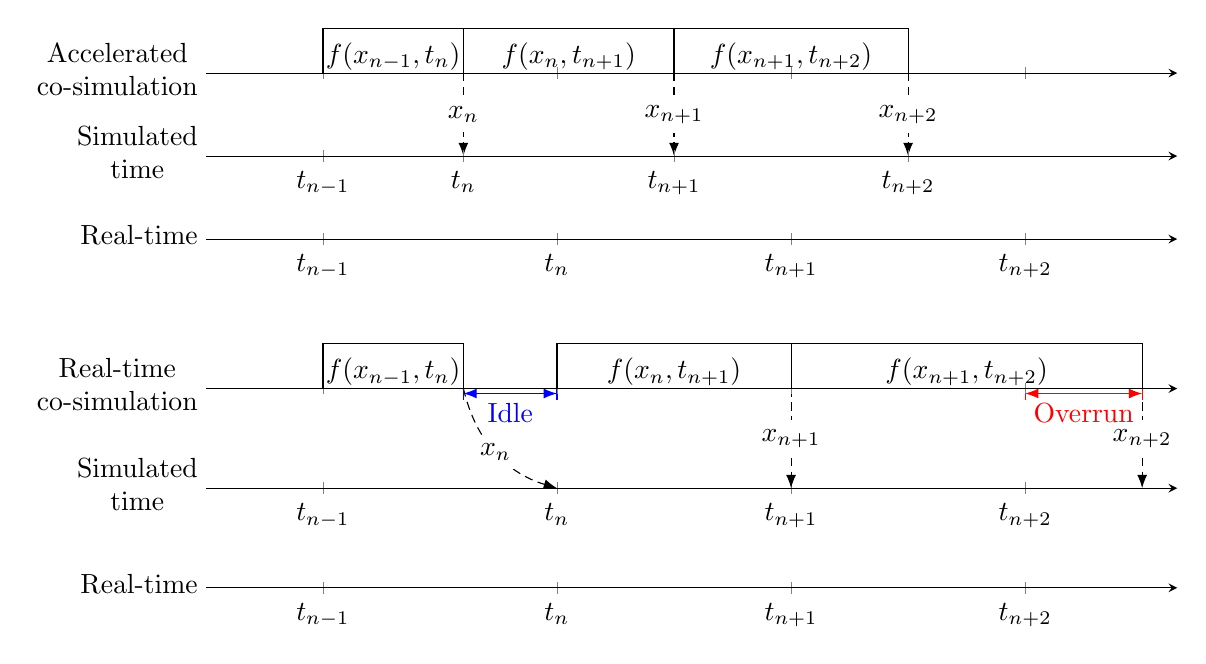
\begin{tikzpicture}[>=Latex]


\begin{axis}[
    xmin=0, xmax=4.15,
    axis x line=bottom,% only show the bottom x axis
    hide y axis,    
    ymin=0,ymax=2.7,
				xticklabels={$t_{n-1}$,$t_{n}$,$t_{n+1}$,$t_{n+2}$},
				xtick={0.5,1.5,2.5,3.5},
				x label style={align=center,at={(current axis.left of origin)},anchor=east, above=0.5mm, left=-0.2mm},
				xlabel={Simulated\\time
				},
				x post scale=1.8
    ]
		\coordinate (u) at (axis cs:0,-.6);
		\coordinate (s) at (axis cs:0,0.6);
		\coordinate (c) at (axis cs:0,2);
		\coordinate (x) at (axis cs:0,2.5);
		\coordinate (y) at (axis cs:0,1.5);
		\path (1.1,0.6) edge[->,densely dashed,bend right] node [align=center,fill=white] {$x_{n}$} (1.5,0);
		\draw [->,densely dashed] (2.5,0.6) -- node [align=center,fill=white] {$x_{n+1}$} (2.5,0);
		\draw [->,densely dashed] (4.0,0.6) -- node [align=center,fill=white] {$x_{n+2}$} (4.0,0);
		
		\draw [<->,blue] (1.1,0.57) -- node [blue,below]{Idle} (1.5,0.57);
		\draw [blue](1.1,0.6) -- (1.1,0.53);
		\draw [blue](1.5,0.6) -- (1.5,0.53);
		
		\draw [<->,red] (3.5,0.57) -- node [red,below]{Overrun} (4,0.57);
		\draw [red](3.5,0.6) -- (3.5,0.53);
		\draw [red](4,0.6) -- (4,0.53);
		
		\node at (0.8,0.7) {$f(x_{n-1},t_n)$};
		\node at (2,0.7) {$f(x_{n},t_{n+1})$};
		\node at (3.25,0.7) {$f(x_{n+1},t_{n+2})$};
		
		\draw [->,densely dashed] (1.1,2.5) -- node [align=center,fill=white] {$x_{n}$} (1.1,2);
		\draw [->,densely dashed] (2,2.5) -- node [align=center,fill=white] {$x_{n+1}$} (2,2);
		\draw [->,densely dashed] (3,2.5) -- node [align=center,fill=white] {$x_{n+2}$} (3,2);
		
		
		
		\node at (0.8,2.6) {$f(x_{n-1},t_n)$};
		\node at (1.55,2.6) {$f(x_{n},t_{n+1})$};
		\node at (2.5,2.6) {$f(x_{n+1},t_{n+2})$};

		
\end{axis}

\begin{axis}[at={(s)},
    xmin=0, xmax=4.15,
    axis x line=bottom,% only show the bottom x axis
    hide y axis,    
    ymin=0,ymax=2,
    scatter/classes={%
        a={mark=o,draw=black}},
				xtick={0.5,1.5,2.5,3.5},
				xticklabels={,,},
				x label style={align=center,at={(current axis.left of origin)},anchor=east, above=0.5mm, left=-0.2mm},
				xlabel={Real-time\\co-simulation},
				x post scale=1.8
    ]
		\addplot+[mark=none,const plot,draw=black]
coordinates
{(0.5,0) (0.5,0.2) (1.1,0.2) (1.1,0)};

\addplot+[mark=none,const plot,draw=black]
coordinates
{(1.5,0) (1.5,0.2) (2.5,0.2) (2.5,0)};

\addplot+[mark=none,const plot,draw=black]
coordinates
{(2.5,0) (2.5,0.2) (4,0.2) (4,0)};

\end{axis}

\begin{axis}[at={(x)},
    xmin=0, xmax=4.15,
    axis x line=bottom,% only show the bottom x axis
    hide y axis,    
    ymin=0,ymax=2,
    scatter/classes={%
        a={mark=o,draw=black}},
				xtick={0.5,1.5,2.5,3.5},
				xticklabels={,,},
				x label style={align=center,at={(current axis.left of origin)},anchor=east, above=0.5mm, left=-0.2mm},
				xlabel={Accelerated\\co-simulation},
				x post scale=1.8
    ]
		\addplot+[mark=none,const plot,draw=black]
coordinates
{(0.5,0) (0.5,0.2) (1.1,0.2) (1.1,0)};

\addplot+[mark=none,const plot,draw=black]
coordinates
{(1.1,0) (1.1,0.2) (2,0.2) (2,0)};

\addplot+[mark=none,const plot,draw=black]
coordinates
{(2,0) (2,0.2) (3,0.2) (3,0)};


\end{axis}

\begin{axis}[at={(c)},
    xmin=0, xmax=4.15,
    axis x line=bottom,% only show the bottom x axis
    hide y axis,    
    ymin=0,ymax=2,
    scatter/classes={%
        a={mark=o,draw=black}},
				xtick={0.5,1.1,2,3},
				xticklabels={$t_{n-1}$,$t_{n}$,$t_{n+1}$,$t_{n+2}$},
				x label style={align=center,at={(current axis.left of origin)},anchor=east, above=0.5mm, left=-0.2mm},
				xlabel={Simulated\\time},
				x post scale=1.8
    ]
		

\end{axis}

\begin{axis}[at={(u)},
    xmin=0, xmax=4.15,
    axis x line=bottom,% only show the bottom x axis
    hide y axis,    
    ymin=0,ymax=2,
    scatter/classes={%
        a={mark=o,draw=black}},
				xtick={0.5,1.5,2.5,3.5},
				xticklabels={$t_{n-1}$,$t_{n}$,$t_{n+1}$,$t_{n+2}$},
				x label style={align=center,at={(current axis.left of origin)},anchor=east, above=0.5mm, left=-0.2mm},
				xlabel={Real-time},
				x post scale=1.8
    ]
		

\end{axis}

\begin{axis}[at={(y)},
    xmin=0, xmax=4.15,
    axis x line=bottom,% only show the bottom x axis
    hide y axis,    
    ymin=0,ymax=2,
    scatter/classes={%
        a={mark=o,draw=black}},
				xtick={0.5,1.5,2.5,3.5},
				xticklabels={$t_{n-1}$,$t_{n}$,$t_{n+1}$,$t_{n+2}$},
				x label style={align=center,at={(current axis.left of origin)},anchor=east, above=0.5mm, left=-0.2mm},
				xlabel={Real-time},
				x post scale=1.8
    ]
		

\end{axis}
   
\end{tikzpicture}

\end{document}